\section{First Section} % Sections can be created in order to organize your presentation into discrete blocks, all sections and subsections are automatically printed in the table of contents as an overview of the talk
%------------------------------------------------

\subsection{Subsection Example} % A subsection can be created just before a set of slides with a common theme to further break down your presentation into chunks


% Frame with plain text
\begin{frame}{Lorem ipsum dolor sit amet}
    Lorem ipsum dolor sit amet, consectetuer adipiscing elit. Aenean commodo ligula eget dolor. Aenean massa. Cum sociis natoque penatibus et magnis dis parturient montes, nascetur ridiculus mus. Donec quam felis, ultricies nec, pellentesque eu, pretium quis, sem. Nulla consequat massa quis enim. Donec pede justo, fringilla vel, aliquet nec, vulputate eget, arcu. In enim justo, rhoncus ut, imperdiet a, venenatis vitae, justo. Nullam dictum felis eu pede mollis pretium. Integer tincidunt. Cras dapibus. Vivamus elementum semper nisi. Aenean vulputate eleifend tellus. Aenean leo ligula, porttitor eu, consequat vitae, eleifend ac, enim. Aliquam lorem ante, dapibus in, viverra quis, feugiat a, tellus. Phasellus viverra nulla ut metus varius laoreet. Quisque rutrum. Aenean imperdiet. Etiam ultricies nisi vel augue. Curabitur ullamcorper ultricies nisi. Nam eget dui. Etiam rhoncus. Maecenas tempus, tellus eget condimentum rhoncus, sem quam semper libero, sit amet adipiscing sem neque sed ipsum.
\end{frame}

%------------------------------------------------

% Start a new section (text is displayed on top of a frame)
\section{Section title}

% Frame with items
\begin{frame}{Frame title}
  \begin{itemize}
    \item First level
    \begin{itemize}
      \item Second level
      \begin{itemize}
      \item Third level
    \end{itemize}
  \end{itemize}
\end{itemize}
\end{frame}

%------------------------------------------------

\begin{frame}
\frametitle{Blocks of Highlighted Text}
\begin{block}{Block 1}
Lorem ipsum dolor sit amet, consectetur adipiscing elit. Integer lectus nisl, ultricies in feugiat rutrum, porttitor sit amet augue. Aliquam ut tortor mauris. Sed volutpat ante purus, quis accumsan dolor.
\end{block}

\begin{block}{Block 2}
Pellentesque sed tellus purus. Class aptent taciti sociosqu ad litora torquent per conubia nostra, per inceptos himenaeos. Vestibulum quis magna at risus dictum tempor eu vitae velit.
\end{block}

\begin{block}{Block 3}
Suspendisse tincidunt sagittis gravida. Curabitur condimentum, enim sed venenatis rutrum, ipsum neque consectetur orci, sed blandit justo nisi ac lacus.
\end{block}
\end{frame}

%------------------------------------------------

\begin{frame}
\frametitle{Multiple Columns}
\begin{columns}[c] % The "c" option specifies centered vertical alignment while the "t" option is used for top vertical alignment

\column{.45\textwidth} % Left column and width
\textbf{Heading}
\begin{enumerate}
\item Statement
\item Explanation
\item Example
\end{enumerate}

\column{.5\textwidth} % Right column and width
Lorem ipsum dolor sit amet, consectetur adipiscing elit. Integer lectus nisl, ultricies in feugiat rutrum, porttitor sit amet augue. Aliquam ut tortor mauris. Sed volutpat ante purus, quis accumsan dolor.

\end{columns}
\end{frame}

%------------------------------------------------
\section{Second Section}
%------------------------------------------------

\begin{frame}
\frametitle{Table}
\begin{table}
\begin{tabular}{l l l}
\toprule
\textbf{Treatments} & \textbf{Response 1} & \textbf{Response 2}\\
\midrule
Treatment 1 & 0.0003262 & 0.562 \\
Treatment 2 & 0.0015681 & 0.910 \\
Treatment 3 & 0.0009271 & 0.296 \\
\bottomrule
\end{tabular}
\caption{Table caption}
\end{table}
\end{frame}

%------------------------------------------------

\begin{frame}
\frametitle{Theorem}
\begin{theorem}[Mass--energy equivalence]
$E = mc^2$
\end{theorem}
\end{frame}

%------------------------------------------------

\begin{frame}[fragile] % Need to use the fragile option when verbatim is used in the slide
\frametitle{Verbatim}
\begin{example}[Theorem Slide Code]
\begin{verbatim}
\begin{frame}
\frametitle{Theorem}
\begin{theorem}[Mass--energy equivalence]
$E = mc^2$
\end{theorem}
\end{frame}\end{verbatim}
\end{example}
\end{frame}

%------------------------------------------------

\begin{frame}
\frametitle{Figure}
Code to include your own image as figure~\ref{fig:acis} from the `Figure' directory.
\begin{figure}

\includegraphics[width=0.5\linewidth]{acis}
\caption{Acis logo}
\label{fig:acis}
\end{figure}
\end{frame}

% Frame with text and picture
\begin{frame}{Frame title}
    \begin{columns}[onlytextwidth]\
      % Text on the left
      \begin{column}{.5\textwidth}
        \begin{itemize}
          \item First level
          \begin{itemize}
            \item Second level
            \begin{itemize}
              \item Third level\cite{Weng98}
            \end{itemize}
          \end{itemize}
        \end{itemize}
      \end{column}
      % Picture on the right
      \begin{column}{.5\textwidth}
        \hfill\raisebox{-10cm}[0pt][10cm]{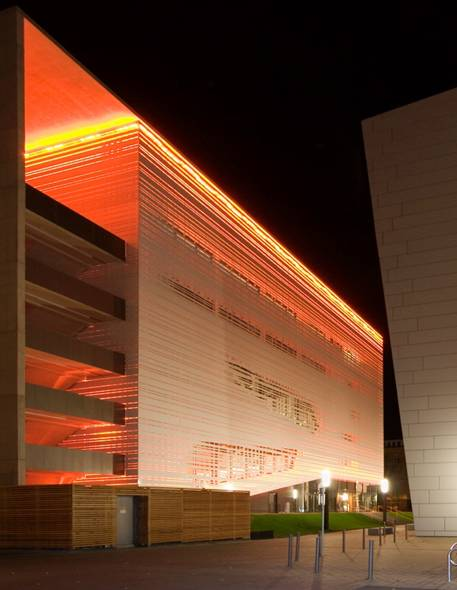
\includegraphics[height=10cm]{figure.jpg}}
      \end{column}
    \end{columns}
    \end{frame}


% Frame with large picture and caption
\begin{frame}
    \begin{figure}
    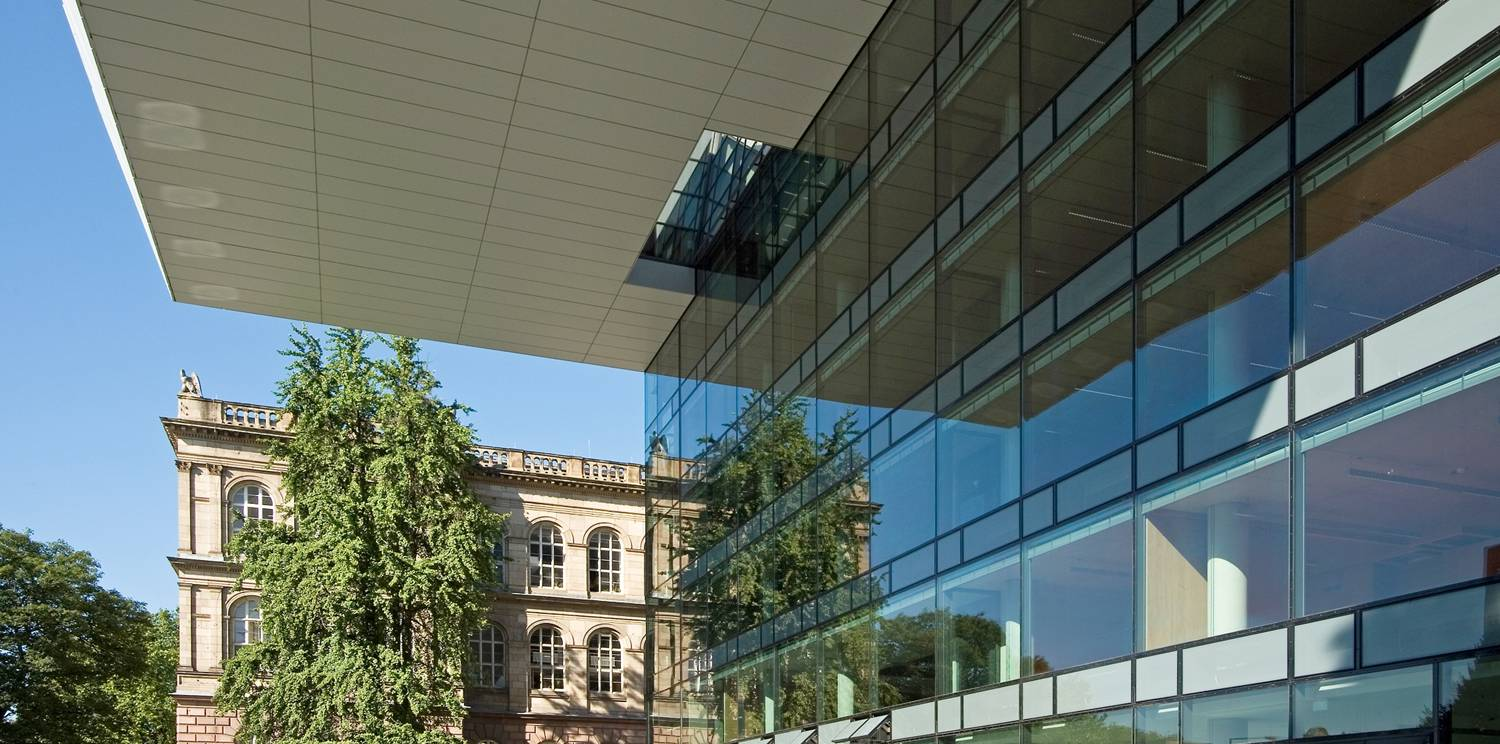
\includegraphics[width=0.7\textwidth]{title_large}
    \caption{Image description}
    \end{figure}
    \end{frame}

%------------------------------------------------

% New section (with charts)
% Note: Using newline in a section is not recommended, this is
% just an example
\section{Section title\newline
Example of a two-line title}

% Frame with horizontal bar chart
\begin{frame}{Add title}
\begin{center}
\begin{tikzpicture}
  \begin{axis}[hor_barchart,symbolic y coords={Kategorie 1,Kategorie 2,Kategorie 3, Kategorie 4},%
               width=0.7\textwidth,height=10cm]
    \addplot [draw opacity=0,fill=rwth-50] coordinates {(4.5,Kategorie 4) (3.5,Kategorie 3) (2.5,Kategorie 2) (4.3,Kategorie 1)};
    \addplot [draw opacity=0,fill=rwth] coordinates {(2.8,Kategorie 4) (1.8,Kategorie 3) (4.4,Kategorie 2) (2.4,Kategorie 1)};
    \legend{Datenreihe 1,Datenreihe 2}
  \end{axis}
\end{tikzpicture}
\end{center}
\end{frame}

% Frame with vertical bar chart
\begin{frame}{Add title}
\begin{center}
\begin{tikzpicture}
  \begin{axis}[ver_barchart,symbolic x coords={Kategorie 1,Kategorie 2,Kategorie 3, Kategorie 4},%
               width=0.7\textwidth,height=10cm]
    \addplot [draw opacity=0,fill=rwth] coordinates {(Kategorie 4,4.5) (Kategorie 3,3.5) (Kategorie 2,2.5) (Kategorie 1,4.3)};
    \addplot [draw opacity=0,fill=rwth-75] coordinates {(Kategorie 4,2.8) (Kategorie 3,1.8) (Kategorie 2,4.4) (Kategorie 1,2.4)};
    \addplot [draw opacity=0,fill=rwth-50] coordinates {(Kategorie 4,3) (Kategorie 3,0.5) (Kategorie 2,5.4) (Kategorie 1,3.4)};
    \addplot [draw opacity=0,fill=rwth-25] coordinates {(Kategorie 4,3.5) (Kategorie 3,1.5) (Kategorie 2,2.2) (Kategorie 1,4.2)};
  \legend{Datenreihe 1,Datenreihe 2,Datenreihe 3,Datenreihe 4}
  \end{axis}
\end{tikzpicture}
\end{center}
\end{frame}

% Frame with pie chart
\begin{frame}{Add title}
\begin{center}
\hspace{2cm}
\begin{tikzpicture}
[
  pie chart,
  slice type={one}{rwth-25},
  slice type={two}{rwth-50},
  slice type={three}{rwth-75},
  slice type={four}{rwth},
  pie values/.style={font={\Large}},
  scale=5
]
  \pie{}{29/one,17/two,23.6/three,30.4/four}
  \legend[xshift=1.5cm,yshift=0.8cm]{{Kategorie 1}/one, {Kategorie 2}/two, {Kategorie 3}/three, {Kategorie 4}/four}
\end{tikzpicture}
\end{center}
\end{frame}

%------------------------------------------------

% Citation
\begin{frame}[fragile] % Need to use the fragile option when verbatim is used in the slide
\frametitle{Citation}
An example of the \verb|\cite| command to cite within the presentation:\\~

This statement requires citation \cite{Weng98}.
\end{frame}